\documentclass[acmsmall,screen,nonacm]{acmart}
\usepackage[T1]{fontenc}
\usepackage{microtype,float,graphicx,booktabs,tabularx,array,ragged2e,tikz,needspace,colortbl,placeins,longtable}
\usetikzlibrary{arrows.meta,positioning,calc}
\settopmatter{printacmref=false,printfolios=true,printccs=true}
\setcopyright{none}
\hypersetup{colorlinks=true,linkcolor=blue!50!black,citecolor=blue!50!black,urlcolor=blue!50!black}
\setlength{\emergencystretch}{2em}
\renewcommand{\topfraction}{.9}\renewcommand{\bottomfraction}{.9}\renewcommand{\textfraction}{.1}
\definecolor{unitshade}{HTML}{ECEFF3}
\providecommand{\doi}[1]{\href{https://doi.org/#1}{doi:#1}}
\newcolumntype{Y}{>{\RaggedRight\arraybackslash}X}
\newcolumntype{L}[1]{>{\RaggedRight\arraybackslash}p{#1}}
\title[Between the Issue and the Warning]{Between the Issue and the Warning: Unspecified Implementation Choices Behind Security Warnings in Agent-Associated Pull Requests}
\author{Arno Strauss}
\affiliation{\institution{School of Computer Science and Applied Mathematics, University of the Witwatersrand}\city{Johannesburg}\country{South Africa}}
\email{2613224@students.wits.ac.za}
\renewcommand{\shortauthors}{Arno Strauss}
\begin{abstract}
Coding agents increasingly turn GitHub issues into pull requests (PRs), so issue text shapes code that static analysis then checks. Controlled studies show that crafted issues can steer agents toward insecure patches, and static analysis has been run on agent patches, but how an issue's requirements relate to the implementation choices behind the warnings in ordinary merged work has not been traced. This paper studies, in the wild, 3,809 recent merged, issue-linked, agent-associated JavaScript/\allowbreak TypeScript task instances (linked issue--PR pairs), 192 of which introduced new findings (reports from static-analysis, dependency and secret scanners), and traces findings to the changed operations behind them. The traced cases show a recurring pattern: the issue asks for a feature, and the PR delivers it through a mechanism the issue never specified, such as a way of turning random bytes into a login verifier that biases the result, although commonly used alternatives existed. Raw finding counts blur this further. In 122 annotated instances, 605 findings map to 322 changed code or dependency operations, and seven instances hold over half the findings but almost none of the source-code operations. In an exploratory matched comparison, issues associated with finding-positive PRs were less explicit about implementation details than those associated with finding-free PRs. In 12 retrospective replays, giving the agent the historical warning coincided with fewer static-analysis alerts and, in one task, a different mechanism, but the replays cannot show why the original choice was made. Public records cannot distinguish repository influence from unseen developer instructions or model behaviour; the exploratory replays motivate better controlled tests of repository context and implementation guidance.
\end{abstract}
\ccsdesc[500]{Software and its engineering~Software creation and management}
\ccsdesc[300]{Security and privacy~Software and application security}
\keywords{Empirical software engineering, coding agents, GitHub issues, security analysis, pull requests, implementation provenance}
\newlength{\crowW}
\newenvironment{casefile}[2]{\par\Needspace{9\baselineskip}\begingroup\footnotesize\renewcommand{\arraystretch}{1.18}\setlength{\crowW}{\dimexpr\linewidth-2.15cm-2\tabcolsep\relax}\noindent\begin{tabular}{@{}>{\bfseries\raggedright\arraybackslash}p{2.15cm}>{\raggedright\arraybackslash}p{\crowW}@{}}\toprule\rowcolor{unitshade}\multicolumn{2}{@{}p{\linewidth}@{}}{\normalsize #1\par\smallskip\scriptsize #2}\\\midrule}{\bottomrule\end{tabular}\endgroup\par\medskip}
\newcommand{\crow}[2]{#1 & #2\\}
\begin{document}
\maketitle
\noindent\textit{2026 BSc Honours research paper. Supervisors: Prof. Michael Pradel (CISPA) and Prof. Hima Vadapalli (Wits).}

\section{Introduction}

Natural language has become an interface to software tools: a plain-text request can now be turned into code changes by a coding agent. On GitHub, an issue is usually a message to a maintainer, in which a user describes a defect or a wanted feature and a person decides how to implement it. Repository-capable coding agents now read the same text as a task, search the repository, edit code and open pull requests (PRs) \cite{b9,b20,b22,b25}, and such PRs appear in large numbers in open-source projects \cite{b11,b21}. Security analysis runs on this work as well: in a dataset of PRs that public signals attribute to coding agents, GitHub's rule-based security bot is among the ten most frequent bot reviewers \cite{b11}. Public issue intake has thereby become an input channel to automated code change.

That channel has a known weakness. Controlled studies show that crafted issue text can steer repair agents toward insecure or vulnerable patches that still pass tests, and that static analysis can miss them \cite{b3,b16}; prompt-injection benchmarks show that tool output and retrieved content can hijack agents, including coding editors \cite{b6,b12,b24}. These studies construct the attack, so they know which operation is responsible and what the issue was meant to cause. Naturally occurring work offers no such ground truth. A public issue--PR link is a starting point, not a record of every instruction or source the implementer saw, and links take several forms, including issues opened after the PR they are linked to \cite{b5}.

What the public record does expose is the outcome: static analysis reports security warnings on agent-associated PRs. How such a warning relates to the task the issue described is largely unexamined. Does it arise in code that implements what was asked, in code that merely accompanies it, or in a dependency change that no one chose? Did the issue say how to implement the feature, or leave that choice open? Existing work studies the pieces separately. Issue-resolution benchmarks judge a patch by running tests \cite{b9}; mining studies characterise agent PRs by size, purpose and acceptance \cite{b11,b21}; and static-analysis research asks whether warnings are actionable and how secure assistant-generated code is \cite{b32,b33,b34,b35}. Closest are studies that run static analysis on agent patches for benchmark issues \cite{b36} and on agent PRs \cite{b37}. Within the studies reviewed in Section~3, none traces warnings in merged, naturally occurring PRs to the changed operation behind them, to its role in the task, and to whether the issue prescribed the mechanism. That is the gap this paper addresses: how issue requirements relate to the implementation choices behind security warnings has not been examined empirically in natural agent-associated work.

A concrete case shows why it matters. An \href{https://github.com/ZHANGTIANYAO1/teamspeak-music-bot/issues/112}{issue} in the teamspeak-music-bot project asks for Spotify as an audio source. The linked \href{https://github.com/ZHANGTIANYAO1/teamspeak-music-bot/pull/118}{pull request} delivers it, and in doing so builds a login verifier by turning each random byte into a character with a remainder operation over a 66-character alphabet. Because 256 byte values do not divide evenly into 66, some characters come up slightly more often than others, and CodeQL reports a biased-random warning. The warning does not say which operation produced it, whether the issue asked for it, or whether a better option existed. The issue asked for Spotify support, not for this way of choosing characters.

I examine this gap in 3,809 merged, issue-linked, agent-associated JavaScript/\allowbreak TypeScript instances, including 192 with newly introduced scanner findings. The analysis uses public issue discussions, PR changes and tool output; these records reveal an implementation without establishing which instructions or context its author saw.

The analysis distinguishes three units often conflated in security reports. First, findings are not changed operations: among 122 initially annotated instances, 605 findings map to 322 operations. Seven instances account for 317 findings, yet 161 of the 166 source-code operations lie outside those seven (Figure~\ref{fig:concentration}). Second, a scanner's reported location need not be the operation responsible for the finding. Third, implementing a requested feature does not mean the issue prescribed its mechanism, as the Spotify case illustrates.

\begin{figure}[!tbp]
\centering
\makebox[\linewidth][c]{\includegraphics[width=1.16\linewidth]{figures/Fig1_Conceptual.pdf}}
\caption{Public evidence connecting a requested task, its linked PR and the scanner's report. The issue--PR connection is conceptual rather than a verified sequence of instructions: an issue can postdate its linked PR, and repository context or private guidance seen by the implementer is not fully observable (Sections~2.1 and~\ref{sec:roles}).}
\label{fig:conceptual}
\end{figure}

\subsection{Research Questions}\label{sec:rqs}

The study moves from the operations behind scanner findings to the wording of the linked issues and the behaviour observed in limited warning-informed replays. Three research questions guide these analyses:
\begin{itemize}
\item \textbf{RQ1.} Which changed operations account for the findings reported on agent-associated PRs, and how do they relate to what the linked issue asked for and to any mechanism that public evidence from before the change prescribed?
\item \textbf{RQ2.} Do issues behind PRs with newly introduced findings differ in how explicitly they are worded from issues behind matched PRs without any?
\item \textbf{RQ3.} In exploratory replays of historical tasks, how do the implementation and CodeQL findings differ when an issue is presented alone, with the historical warning, or with alternative forms of warning-derived safety guidance?
\end{itemize}

\subsection{Contributions}

The study contributes a finding-to-change evidence map, an operation-level classification of how changes serve public requests, and source-linked examples distinguishing requested functionality from the mechanisms used to implement it. Matched issue comparisons and warning-informed replays provide narrower complementary evidence. The coding protocol, quality-control decisions and limits on inference are described in Sections~\ref{sec:attrib},~\ref{sec:roles} and~\ref{sec:threats}.

\section{Background}

\subsection{Tasks, Patches and Coding Agents}

GitHub issues record requested functionality, defects and discussion; PRs record proposed changes. Their links permit analysing a request alongside a patch, but do not prove that the public issue initiated, fully specified or dictated the implementation \cite{b5}. Coding agents may also use repository instructions, files and tool output absent from the public issue \cite{b20,b22}. \emph{Agent-associated} means that public PR metadata, branch patterns or issue/PR text indicate coding-agent involvement; a tool mention does not prove agent authorship, so the sample is not a census of autonomously written patches.

\subsection{Warnings, Advisories and Retained Findings}

CodeQL (queries over a code database \cite{b44}) and Semgrep report static-analysis warnings on source code. OSV and Trivy report vulnerable dependencies, and Gitleaks flags possible secrets. Any retained result from these tools is called a \emph{finding}, and \emph{warning} is kept for source-code diagnostics. An \emph{alert} is one CodeQL or Semgrep result at a single revision. A warning counts as introduced if it appears after the PR but not before, and RQ3 counts CodeQL alerts.

An instance is \emph{finding-positive} if its PR newly introduced at least one finding, and \emph{finding-negative} if it introduced none under the checks that applied and completed. A check that did not apply, was unavailable or failed is not read as a negative result. Neither label shows that older findings are absent, that an exploit exists, or that the code works.

\subsection{Task Relevance and Mechanism Choice}

\emph{Task role} records whether a changed operation directly implements the request or accompanies that work through code, dependencies, configuration or tests, including incidental implementation choices the issue did not request. \emph{Mechanism prescription} asks whether the issue specified the operation itself.

\section{Related Work}

\subsection{Coding Agents and How They Are Judged}

SWE-bench turned issue resolution into a benchmark: 2,294 tasks from 12 Python repositories, where a patch counts as correct if the repository's tests pass \cite{b9}. SWE-agent, AutoCodeRover and OpenHands are agents built to navigate a repository, edit code and run tests on such tasks \cite{b22,b25,b20}. They answer whether the requested behaviour works. They do not ask which operations a patch used to get there, or what static analysis says about those operations. The SWE-bench authors themselves point out that static analyzers could be run on generated patches \cite{b9}. Sajadi et al. did so for patches that a language model and three agent frameworks generated for SWE-bench issues, using Semgrep, Bandit and CodeQL, and found vulnerabilities more likely in patches that touched more files and in issues without code snippets or details of expected behaviour \cite{b36}. That setting is a benchmark of generated, unmerged patches. This paper runs security analysis on merged, naturally occurring agent-associated PRs and asks which changed operation produced each warning.

\subsection{Agent Pull Requests and Issue Mining}

Coding agents already contribute pull requests at scale. AIDev collects 456,535 PRs attributed to five agents through public signals such as bot authors, branch prefixes and co-authorship messages, and finds that they are accepted less often and are structurally simpler than human PRs \cite{b11}. A study of 567 Claude Code PRs in 157 projects compares them with human PRs on size, purpose and acceptance \cite{b21}. Neither looks at security findings. Siddiq et al. study how maintainers review 1,293 security-related agentic PRs \cite{b38}, and Rabbi et al. ran Semgrep on baseline and PR commits of 675 security-related PRs, finding that about 15\% introduced at least one issue, most often inefficient regular expressions, command injection and path traversal \cite{b37}. Both start from PRs that are about security. This paper starts from ordinary issue-linked work, where a warning is a side result of the feature. The study relies on similar public signals, plus weaker markers on the issue side, so its PRs are called agent-associated and not agent-written (Section~2.1).

Issue studies describe what users ask for in open-source AI repositories \cite{b23}, which issues suit newcomers \cite{b26}, and how issues and PRs connect \cite{b5}. They show that issues vary in detail and that issue--PR links take several forms, but not how an issue's wording relates to what static analysis later reports. Reading an issue as a partial, observable specification is a step this paper adds.

\subsection{Crafted Issues and Untrusted Context}

Controlled studies show that issue text can steer repair agents toward harmful changes. Przymus et al.\ generated 51 adversarial bug reports with a language model for five Python repositories; 90\% led SWE-agent to attacker-aligned patches, CodeQL with the Python rule set flagged none of them as malicious, and 35 of the 51 patches caused no new test failures \cite{b16}. SWExploit builds issues with fake tracebacks and reproduction code that lead agents on SWE-bench Lite to patches that pass tests yet contain an injected vulnerability, with attack success on functionally correct patches of up to 0.91 in the settings it evaluates \cite{b3}. Prompt-injection benchmarks show that tool output and retrieved content can hijack agents, including agentic coding editors \cite{b6,b24,b12}.

In all of these the attacker builds the input, so the responsible operation is known from the start. In ordinary repositories nobody knows it, and nobody knows what role the issue played. This paper studies that setting. Adversarial input cannot be ruled out, and how common it is goes unmeasured.

\subsection{Static-Analysis Warnings and Generated Code}

Warnings from static analysis are read with care by the people who receive them. Developers name false positives and the way warnings are presented among the reasons they avoid such tools \cite{b33}, and a body of work tries to separate actionable warnings from the rest, although reported accuracy can be inflated by data leakage and unreliable labels \cite{b34}. For assistant-generated code, one line of work prompts assistants with vulnerability-prone scenarios and checks what they write \cite{b35}, and controlled studies examine the security of code written with an assistant \cite{b41} and compare Copilot's vulnerabilities with human-introduced ones \cite{b42}. In secure code review, one static analysis tool flagged the vulnerable function in 52\% of vulnerability-contributing commits, and at least 76\% of warnings in vulnerable functions were unrelated to the commit \cite{b43}, which is why warnings here are tied to the changed operation. Another analyses code attributed to Copilot in GitHub projects, where static analysis flagged about a quarter of the snippets as security-weak \cite{b32}.

These studies connect warnings to snippets or to assistant output. None traces a warning on a merged agent-associated PR back to the changed operation behind it and to the issue that asked for the work, and none treats the warning count as something to take apart. This paper does that for one cohort.

\subsection{Research Gap}

Taken together, the earlier work shows four things. Agents can implement GitHub issues, and are judged by whether tests pass \cite{b9,b20,b22,b25}. Agent PRs are common and have been studied for size, purpose and acceptance \cite{b11,b21}. Crafted issues and injected context can push agents toward insecure patches, with the responsible operation known by construction \cite{b3,b16,b6,b12,b24}. And static analysis can flag security weaknesses in assistant-generated code, in agent patches for benchmark issues and in security-related agent PRs \cite{b32,b35,b36,b37}, with vulnerabilities in the benchmark setting more likely when issues lacked detail \cite{b36}, which gives RQ2 a prior.

What is missing is how, in natural agent-associated work, what an issue asks for relates to the implementation choices behind security warnings. That has three parts: which changed operation accounts for a warning, given that many reports can follow from one change; whether that operation implements what the issue asked for or only comes along with it; and whether the issue prescribed the mechanism or left the choice open. Answering them needs the issue, the patch and the warning side by side, which is what the research questions in Section~\ref{sec:rqs} do. The gap is claimed only against the studies reviewed here.

\section{Study Design and Methods}

I conduct an empirical, observational study of public GitHub issues linked to merged, agent-associated pull requests (PRs) in open-source JavaScript and TypeScript repositories. The analysis follows the evidence from a requested task to the merged patch and the security findings recorded by static-analysis, dependency and secret-scanning tools. It has four stages: (1) select issue--PR instances and compare scanner results before and after the PR; (2) map retained findings to changed operations, then characterise how those operations relate to the issue (RQ1); (3) compare issue wording with matched scanner-negative instances (RQ2); and (4) examine a small set of retrospective, warning-informed replays (RQ3). Figure~\ref{fig:overview} separates the observational comparisons from the replay study.

The units of analysis differ. A \emph{task instance} is one sampled issue--PR link; a \emph{finding} is one retained scanner report; a \emph{responsible change} is the changed operation to which a finding is attributed; and an \emph{implementation choice} groups related changes within an instance. RQ2 uses matched pairs of instances. RQ3 compares generated patches for selected tasks. These units are kept distinct throughout.

\begin{figure}[!tbp]
\centering
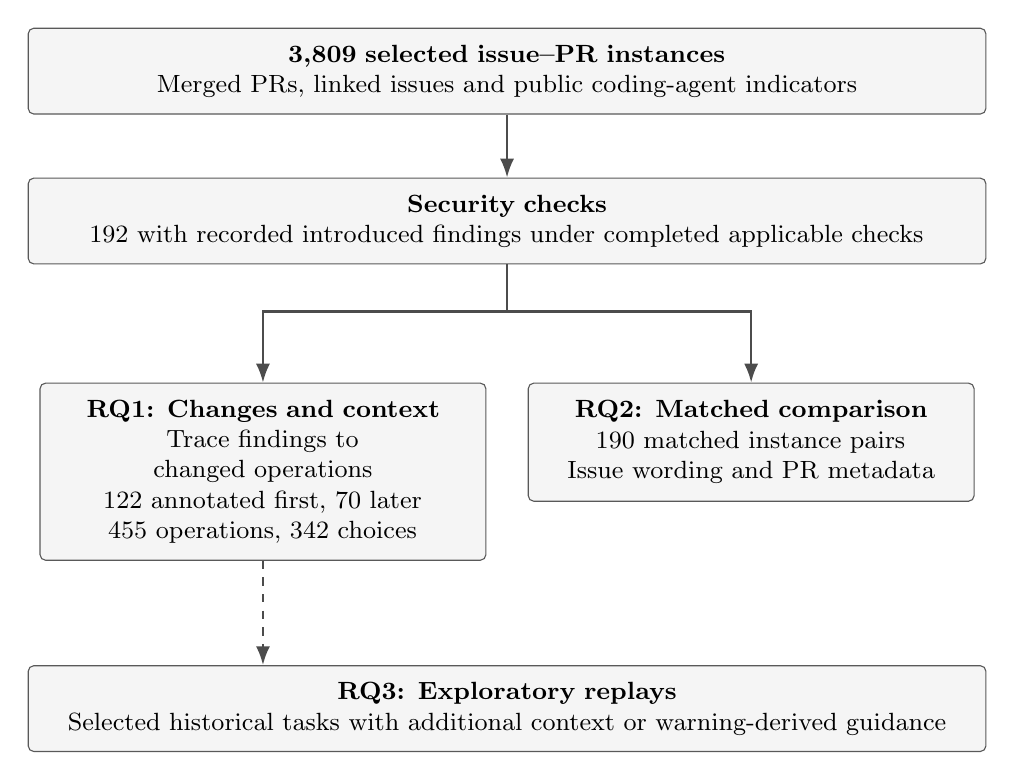
\begin{tikzpicture}[
  font=\small,>={Latex[length=2.4mm]},
  base/.style={draw=black!65,fill=black!4,rounded corners=2pt,align=center,inner xsep=8pt,inner ysep=6pt},
  wide/.style={base,text width=11.6cm},
  panel/.style={base,text width=5.1cm,minimum height=1.5cm},
  link/.style={->,line width=.9pt,draw=black!70},
  weak/.style={->,dashed,line width=.9pt,draw=black!70}]
  \node[wide] (cohort) {\textbf{3,809 selected issue--PR instances}\\ Merged PRs, linked issues and public coding-agent indicators};
  \node[wide,below=8mm of cohort] (checks) {\textbf{Security checks}\\ 192 with recorded introduced findings under completed applicable checks};
  \node[panel,anchor=north] (rq1) at ($(checks.south)+(-3.1cm,-1.5cm)$) {\textbf{RQ1: Changes and context}\\ Trace findings to changed operations\\ 122 annotated first, 70 later\\ 455 operations, 342 choices};
  \node[panel,anchor=north] (rq2) at ($(checks.south)+(3.1cm,-1.5cm)$) {\textbf{RQ2: Matched comparison}\\ 190 matched instance pairs\\ Issue wording and PR metadata};
  \node[wide,anchor=north] (rq3) at ($(rq1.south)!0.5!(rq2.south)+(0,-1.7cm)$) {\textbf{RQ3: Exploratory replays}\\ Selected historical tasks with additional context or warning-derived guidance};
  \draw[link] (cohort) -- (checks);
  \draw[line width=.9pt,draw=black!70] (checks.south) -- ++(0,-6mm) coordinate (fork);
  \draw[link] (fork) -| (rq1.north);
  \draw[link] (fork) -| (rq2.north);
  \draw[weak] (rq1.south) -- (rq1.south |- rq3.north);
\end{tikzpicture}
\caption{Study overview: the sampled population, the RQ1 attribution, the RQ2 matched comparison and the RQ3 replays. The dashed arrow shows that the replay tasks come from historical instances with CodeQL findings; RQ3 does not use the RQ2 pairs.}
\label{fig:overview}
\end{figure}

\subsection{Population and Selection}

Discovery searched GitHub for merged PRs linked to issues (qualifiers \texttt{is:pr}, \texttt{is:merged}, \texttt{linked:issue}) in non-archived JavaScript/\allowbreak TypeScript repositories with at least 100 stars, merged between 1 November 2025 and 11 August 2026. JavaScript and TypeScript match the CodeQL and Semgrep rule sets applied, the start date keeps the sample recent, and the star cutoff excludes very small repositories. The snapshot contains 3,809 distinct issue--PR instances in 723 repositories (609 JavaScript, 3,200 TypeScript; selection criteria and cohort characteristics in Table~\ref{tab:cohort}). Agent indicators include PR authorship or metadata, branch and description markers, and weaker issue-side references to Codex, Copilot, Cursor, Claude or Devin; for 236 instances the only association is an issue-side marker, not PR-side evidence. The 100-star threshold is a practical popularity filter rather than a quality measure; related studies of agent PRs also use this cutoff \cite{b37,b38}. Stars and language are snapshot metadata, not values reconstructed at each merge date. The cohort is neither a random GitHub sample nor an estimate of finding prevalence among all coding-agent work.

\subsection{Detecting and Retaining Introduced Findings}

The pipeline records scanner applicability, execution and findings separately (Section~2.2). CodeQL and Semgrep findings are counted as introduced when the archived comparison reports them after, but not before, a PR. For the original cohort, retained source-code findings also have a primary or data-flow location on a PR-added line. These are \emph{introduced reports}, not independently established new vulnerabilities: a changed data-flow path may affect an existing flagged statement (Table~\ref{tab:scanners}).

Dependency results received an additional merge-base verification in the first annotation cohort. Package/version records were compared at the PR's true merge base and head; this verification excluded 12 initially positive instances after four earlier exclusions. Section~\ref{sec:s2} reports the checks and their results. Equivalent verification is not established for all 70 subsequently annotated positives, so I do not generalise the stronger verification claim to them.

Within the snapshot, 192 instances had at least one newly introduced finding, whereas 3,617 had none recorded. The latter group was not necessarily assessed by every available scanner. Of the 192 positives, 191 have at least one mapped change; one instance with 61 unmapped findings stays in the instance denominator but not the change denominator. Detailed annotation first covered 122 positive instances; 70 were added later. The first 122 were an annotation batch rather than a randomly selected sample of the 192 positives. The two groups contain 322 and 133 mapped operations (455 in total). The 605 findings reported below belong to the original 122-instance cohort only.

\subsection{Deduplication and Finding-to-Operation Attribution}\label{sec:attrib}

A reported finding is not itself the changed operation: the scoped-package regex added in T3Code, for example, is associated with two distinct CodeQL rules that concern one regex-based strategy (Section~\ref{sec:s3}). Deduplication merged repeated records of a finding within an instance without merging distinct rules or advisories, yielding 605 findings from 832 raw tool references in the 122-instance cohort. For source-code warnings the comparison used reported rules and locations, changed hunks and available pre-change code; for dependency findings it used declared or resolved versions before and after the PR. A reported file location alone did not establish the responsible operation; Table~\ref{tab:mapping} gives the mapping basis of every finding.

I use model-assisted annotation to connect each retained finding to a changed code, configuration or dependency operation. The model received the scanner finding, tool evidence and PR diff, but not the issue text or PR description. A candidate link was retained only when the record identified a changed file, a line or diff hunk, and an explanation of how that change accounts for the finding. The check establishes a traceable \emph{evidence basis}; it is not independent human confirmation of every link.

For 142 dependency findings in the original cohort, recorded merge-base verification supports the package/version attribution; 36 of these links were resolved during that verification. After exclusions, the 122-case workbook records 605 retained findings mapped to 322 changes (Table~\ref{tab:mapping}). The underlying dependency verification records and counts are given in Section~\ref{sec:s2}.

The recorded annotation model was GPT-5.6 Sol with medium reasoning effort. This model-assisted stage has no independent per-link second-annotator agreement estimate. One changed operation can account for several findings, so a finding count cannot be read as a count of implementation decisions. Subsequent task-role coding compares the mapped change with the issue's requested goals; it does not independently revalidate the finding-to-change link (Section~\ref{sec:roles}). Case evidence is presented in Sections~\ref{sec:s3} and~\ref{sec:s6}.

Figure~\ref{fig:rq1-method} shows the pipeline from scanner findings through evidence-gated mapping to task-role coding and grouped implementation choices. Model-assisted grouping of the 455 changes yields 342 choices within instances. Each receives an origin label H, T, M or U based on pre-change evidence (Table~\ref{tab:m1}); M choices also receive a separate explanation tier (T1--T5; Table~\ref{tab:rules-full}).

\begin{figure}[!tbp]
\centering
\includegraphics[width=0.9\textwidth]{figures/RQ1_Methodology.pdf}
\caption{Mapping findings to responsible changes and then to implementation choices. A blue bar at the left of a box marks a model-assisted step. Teal dashed callouts provide admissible evidence (the diff, issue or pre-introduction context); red marks an unsupported mapping or later evidence excluded from origin coding. Heavy dark outlines mark retained counts; the dashed final box denotes explanation tiers considered only for M choices. The yes/no arrows show the evidence gate, not a statistical test. A proposed finding-to-change link is retained only with a changed file, line or hunk, and supporting explanation (Table~\ref{tab:m1}).}
\label{fig:rq1-method}
\end{figure}

As a worked example, in Case~3 (Section~\ref{sec:rq1-open}) CodeQL's file-system-race report is the finding, the check-then-read sequence the PR added is the responsible change, and the read is Direct although the issue does not prescribe that sequence, so task role and implementation mechanism need separate annotations.

\subsection{Task Role, Artifact Context and Public Antecedents}\label{sec:roles}

Task role was coded per change by comparing a factual operation summary with the issue's requested goals (Table~\ref{tab:m1}). The labels (Direct, Supporting, Unclear) describe the operation's role, not whether its mechanism was publicly prescribed or who chose it, so a sanitisation step chosen inside a requested feature can be Supporting. The annotations also record a finding family and an affected artifact: production source, tests or fixtures, documentation or examples, a dependency manifest, or a generated lockfile. The artifact category is recorded for the finding's reported location, such as a warning's primary location, which need not be the file that contains the mapped change. A pattern in a test or README does not imply the exposure of the same pattern in deployed code.

For the original 322 changes, an initial model-assisted pass assigned task roles using the frozen issue request and the change evidence, without PR-description text or complete finding records. A subsequent source-assisted quality-control pass revised 11 roles (seven Direct to Supporting and four Supporting to Direct); the workbook retains the earlier and final labels and case-specific reasons. These corrections do not constitute a second-annotator agreement study or independent revalidation of all links. The 133 later changes also have model-assisted roles.

A separate model-assisted grouping combines 455 changes into 342 implementation choices and codes their public origin as H (publicly prescribed), T (mechanical), M (a mechanism selected among alternatives) or U (unresolved). The explanation tiers for M choices characterise observable antecedents, not private agent reasoning. The reported route counts use one frozen classification snapshot (Table~\ref{tab:routes}); a preceding snapshot is retained there as a sensitivity record. These aggregate labels have not undergone an independent blind human reliability assessment.

Public antecedents were judged against the recorded introduction chronology. A pre-existing helper or discussion is a possible source, not evidence that the contributor viewed it. Issue timestamps can postdate PR creation: in the original 122 instances, 4 PRs were opened before their linked issue and 15 more within 10 minutes after it. These are PR creation times, not the time the implementing code first appeared, and the public issue may omit private user or agent messages. A link between an issue and a PR thus does not show that the agent worked from that issue, and a Direct role records semantic alignment with the public issue's goals, not that the issue preceded, initiated or caused the change. Neither an absent antecedent nor a mechanism's first appearance in a patch therefore establishes autonomous invention.

\begin{table}[!tbp]
\caption{RQ1 decision rules and non-equivalences. Task role is decided per responsible change; the origin per grouped choice.}
\label{tab:m1}
\fontsize{8}{10}\selectfont\renewcommand{\arraystretch}{1.1}
\begin{tabularx}{\linewidth}{@{}L{2.5cm}YY@{}}
\toprule
\textbf{Code} & \textbf{Affirmative decision rule} & \textbf{Crucial boundary}\\
\midrule
\multicolumn{3}{@{}l}{\textit{Task role (per responsible change)}}\\
\textbf{Direct} & Implements a substantive goal of the public issue. & The issue need not prescribe the mechanism.\\
\textbf{Supporting} & Enables or accompanies the requested work rather than fulfilling it, including incidental implementation choices the issue did not request. & Role is not inferred from file type alone.\\
\textbf{Unclear} & Evidence cannot establish the task relation. & Uncertainty is retained, not forced into a binary.\\[2pt]
\multicolumn{3}{@{}l}{\textit{Mechanism origin (per implementation choice)}}\\
\textbf{H: prescribed} & Pre-introduction public evidence specifically fixes the mechanism. & A broad goal or later evidence is insufficient.\\
\textbf{T: mechanical} & Dependency resolution, generated artifacts or tooling produce the choice. & Not evidence of discretionary choice.\\
\textbf{M: alternatives} & A concrete mechanism is used though plausible alternatives exist and public evidence did not fix it. & Precedent can explain M; M is not proof of invention.\\
\textbf{U: unresolved} & Evidence cannot separate H, T and M. & Missing evidence is not proof of choice.\\
\midrule
\textbf{Public antecedent} & For M choices: pre-change reuse, precedent, explicit contract or contextual support; ``none'' only after the bounded evidence review. & A public source's existence does not prove the contributor saw it.\\
\bottomrule
\end{tabularx}
\end{table}

\subsection{Matched Controls and Issue Coding}\label{sec:rq2-design}

RQ2 compares how issues are worded in finding-positive instances and in matched controls with no newly introduced finding under the checks that applied and completed. A control is not thereby secure: it may carry older findings, and not every tool ran on it. A frozen matcher that never saw outcomes paired each positive with at most one control. It used completed check opportunity, a 90-day window on PR creation date, and bounds of about fourfold on changed lines and files, and it preferred a control from the same repository (same-repository) to one from another (cross-repository). Issue wording, review variables, agent identity and security labels played no part (Figure~\ref{fig:rq2-method}; protocol in Section~\ref{sec:s5}). Of the 192 positives, 190 were matched (115 same-repository, 75 cross-repository; Table~\ref{tab:rq2-diag}). These are frozen matching records and not a rerun of the optimisation. Matching does not equate the tasks or randomise the wording.

Each issue received one of three wording labels: Problem only, Suggests solution or Explicit instruction. They describe the specificity of wording, not whether a security requirement was stated or the exact mechanism prescribed; Explicit instruction is not the choice-level H origin. One asymmetry is not removed by pairing: positive-side labels were frozen in earlier annotation stages, whereas control labels were produced later from blinded packets that withheld analysis outcomes and pair identities, and cross-pass agreement was not computed, so a difference between coding passes, not only between issue texts, could contribute to the paired contrast (see Section~\ref{sec:threats} for annotation limitations). The 121 original-cohort pairs and the 115 same-repository pairs are nested sensitivity subsets, not independent replications. The matched pair is the unit of analysis. I use a paired Stuart--Maxwell test to compare the three issue-wording categories. The primary test was recomputed from its frozen contingency table (Table~\ref{tab:rq2}); the Holm adjustment within a family of nine comparisons and the secondary comparisons are taken from the archived analysis (Section~\ref{sec:s5}). Matching does not equate task content or other unmeasured differences and cannot undo the non-random selection of the cohort, so the comparison describes an association and cannot identify a causal effect of instructions.

\subsection{Retrospective and Information-Guided Replays}\label{sec:rq3-design}

The RQ3 replays are a retrospective diagnostic, separate from the RQ2 pairs (Figure~\ref{fig:rq3-method}; definitions in Table~\ref{tab:m2}). For 14 historical tasks there were three inputs: O, the original issue; W, the issue plus the historical CodeQL warning; and P, the issue plus a security property derived from the warning without naming its rule. W and P use hindsight, so they could not be given to an agent in advance. Every task has a historical CodeQL warning, which W needs, and the 14 tasks are a selected set, not a sample of finding-positive instances. Of 42 intended outputs, 40 were kept (12 O, 14 W, 14 P), which gives 12 complete O/W/P triples. The two missing O arms were not filled in. Each arm is one archived generation. A read-only check of the recovered research master found 40 archived analysis records and 40 baseline links with recorded input hashes. The historical analysers were not rerun, and task correctness was not tested.

A separate earlier screen retained 195 patch versions across 65 implementation-choice tasks: 19 tasks were scanner-positive in at least one stage and seven in all three. Those seven entered the later P1--P5 guidance pilot, not the separately selected 14-task O/W/P series. The stages are not verified independent generations, and conflicting pilot-run records preclude using P1--P5 as a main result (Section~\ref{sec:s6}).

Figure~\ref{fig:rq3-method} shows the two protocols as separate branches that are not pooled. In each, a task forks into arms that share the original issue and pre-PR snapshot and differ in added information; a model generates one patch per arm, which CodeQL scans. New alerts, and alerts sharing the historical rule, are counted against the recorded baseline on the 12 complete triples (Table~\ref{tab:replays}).

\begin{figure}[!tbp]
\centering
\includegraphics[width=0.78\textwidth]{figures/RQ3_Methodology.pdf}
\caption{RQ3: two separate exploratory replay protocols, never pooled. Each task is generated once per arm from the same issue and pre-PR snapshot, with different information added: the original issue (O), plus the historical CodeQL warning (W), or plus a safety property derived from it (P). P1--P5 are five further guidance conditions (Table~\ref{tab:m2}). Amber marks input derived with hindsight.}
\label{fig:rq3-method}
\end{figure}


\section{Results}

RQ1 is the main analysis (Sections~\ref{sec:rq1-roles} and~\ref{sec:rq1-open}); RQ2 and RQ3 (Sections~\ref{sec:rq2-res} and~\ref{sec:rq3-res}) are secondary. The provenance of mappings, task roles and origins is given in Sections~\ref{sec:attrib} and~\ref{sec:roles}.

\subsection{RQ1: Findings Versus Changed Operations}\label{sec:rq1-roles}

Because one responsible change can trigger several scanner reports, raw finding totals can overstate the number of distinct code or dependency operations. I examine this in the first 122 finding-positive instances annotated, an initial cohort rather than a random sample of all 192 positives. These instances contain 605 findings mapped to 322 responsible changes (1.88 findings per change). The cohort illustrates this relationship but does not establish its prevalence across agent-associated development. Findings are concentrated: seven instances contain 317 of the 605, and 228 of those 317 are dependency-related (Table~\ref{tab:concentration}). In spec-workflow-mcp, a \href{https://github.com/Pimzino/spec-workflow-mcp/pull/173}{pull request} that fixes a path-translation failure also refreshes the lockfile, and its 131 retained dependency-related reports map to 36 operations.

Figure~\ref{fig:concentration} compares the weight of those seven instances in findings with their weight in changed operations.

\begin{figure}[!tbp]
\centering
\includegraphics[width=0.7\linewidth]{figures/Fig5_Concentration.pdf}
\caption{A few instances hold many findings but almost none of the source-code changes. Each bar splits one total between the seven instances with the most findings and the other 115 in the original cohort. The seven hold 52\% of all findings but only 3\% of source-code responsible changes. Counts for the seven are the totals minus the excluded-seven counts in Table~\ref{tab:concentration}.}
\label{fig:concentration}
\end{figure}

Seven instances carry 52\% of the findings and 3\% of the source-code changes. Excluding the seven instances leaves 115 instances, 288 findings and 211 changes (1.36 findings per change). Source-code findings fall from 294 to 205, but their changes only from 166 to 161, while dependency-related findings fall from 293 to 65. The seven are propagation-heavy rather than uniformly dependency-heavy: five owe their counts to dependency fan-out, and two GSD instances chiefly to data-flow reports, which contribute 89 source-code findings but only five changes. So 161 of the 166 source-code changes lie outside the seven. Fan-out from a single dependency change is a familiar source of inflated counts. The point here is that it is almost absent from source-code operations.

Task roles differ by finding family (Table~\ref{tab:role}). Source-code changes divide evenly between Direct and Supporting under this codebook, whereas dependency advisories are mainly Supporting. Supporting includes incidental choices inside requested features (Section~\ref{sec:roles}), so it does not imply peripheral work or identify who selected a mechanism.

\begin{table}[!tbp]
\caption{Findings and responsible changes by finding family and task role.}
\label{tab:role}
\small
\begin{tabular}{@{}l>{\columncolor{unitshade}}r@{\hspace{10pt}}rrrr@{}}
\toprule
& \multicolumn{1}{>{\columncolor{unitshade}}c}{\textbf{Findings}} & \multicolumn{4}{c}{\textbf{Responsible changes (task role)}}\\
\cmidrule(l{2pt}r{2pt}){2-2}\cmidrule(l){3-6}
\textbf{Finding family} & \multicolumn{1}{>{\columncolor{unitshade}}r}{Reported} & \textbf{Total} & Direct & Supporting & Unclear\\
\midrule
Source-code warnings & 294 & \textbf{166} & 82 & 82 & 2\\
Dependency advisories and downgrades & 290 & \textbf{137} & 4 & 132 & 1\\
Secret-like findings & 18 & \textbf{16} & 3 & 13 & 0\\
Other dependency-version changes & 3 & \textbf{3} & 2 & 1 & 0\\
\midrule
Total & 605 & \textbf{322} & 91 & 228 & 3\\
\bottomrule
\end{tabular}
\par\smallskip\raggedright\footnotesize Original 122 finding-positive instances. A finding is one deduplicated tool report; a responsible change is the changed operation to which one or more findings were mapped, and task role is coded per responsible change. Not the extended 455-change population (Section~\ref{sec:s4}).
\end{table}

A finding's reported location is not always the changed operation. Of the 294 source-code findings, 135 were mapped through the tool's primary location on a PR-added line and 159 through a data-flow or related location on an added line (Section~\ref{sec:attrib}). In post-hoc sensitivity checks using the original workbook, excluding all 159 flow-mapped findings leaves 446 findings and 285 mapped changes; excluding instead the ten instances with issue-side-only agent markers leaves 580 findings and 302 changes. Applying both restrictions leaves 428 findings and 268 changes. Among the 147 source-code changes in the PR-side-marker subset, task roles are 66 Direct, 79 Supporting and two Unclear. Thus the finding-to-change distinction survives both restrictions, while the exact 82/82 role split does not. The 159 trace to 37 changes in 32 instances, and two GSD instances contribute 86 of them. In those instances, a test for shutdown-signal handling and a test for recovering an interrupted completion step each create a temporary path; CodeQL reports 42 and 44 insecure-temporary-file findings in other repository files that the data flow from these paths reaches, so two test operations account for 86 reports (Section~\ref{sec:s3}). Because an added data-flow step can make a previously flagged statement appear in a before/after comparison (Table~\ref{tab:scanners}), these 86 may include existing reported sinks; they are mapped reports, not evidence of 86 newly exposed sinks. Counting such findings by reported location spreads one change's warnings across many places.

Artifact context also changes what a finding warrants. A Paperclip \href{https://github.com/paperclipai/paperclip/pull/5240}{pull request} contains two file-system-race warnings, both reported in and mapped to added test code, and a dot-ai \href{https://github.com/vfarcic/dot-ai/pull/286}{pull request} triggers Gitleaks on an instructional token placeholder in a README, which is a documentation finding rather than a usable credential (Section~\ref{sec:s3}). In the extended population of 455 changes, the same rule also spans tests and production code (Figure~\ref{fig:scanner}; Section~\ref{sec:s4}); those counts come from archived records and the 133 later roles are model-assisted.

\subsection{RQ1: Requested Behaviour Versus Implemented Mechanism}\label{sec:rq1-open}

A Direct role says that an operation implements what the issue asked for, not that the issue chose how. The cases below show what that means in practice. The three cases illustrate distinct ways in which a requested feature and its security-relevant implementation can diverge. They are explanatory examples, not a prevalence sample. Each card identifies the request, the implemented operation, the resulting warning, an alternative approach and the limits of what public evidence can establish. Rule names, line numbers and links to the exact code are in Section~\ref{sec:s3}.

\begin{casefile}{\textbf{Case 1: Spotify login verifier}\ \ {\scriptsize\texttt{ZHANGTIANYAO1/\allowbreak teamspeak-music-bot}}}{\href{https://github.com/ZHANGTIANYAO1/teamspeak-music-bot/issues/112}{Issue \#112}\ \ \href{https://github.com/ZHANGTIANYAO1/teamspeak-music-bot/pull/118}{PR \#118}}
\crow{Request}{Add Spotify as an audio source next to existing music services. The issue suggests a solution but says nothing about how the login verifier is built.}
\crow{What the PR did}{Builds the verifier by turning each random byte into a character with a remainder operation over a 66-character alphabet. 256 is not a multiple of 66, so some characters are slightly more likely.}
\crow{Warning}{CodeQL: biased random value in a cryptographic setting.}
\crow{Reading}{The change implements the requested Spotify service and is classified as Direct, but the issue did not prescribe how to generate the verifier. The resulting bias is small; the case illustrates an implementation-level warning, not a claim of severe exploitation.}
\crow{Better option}{Encode the random bytes in a standard URL-safe form, which is what the PKCE specification describes \cite{b39}, or discard out-of-range bytes before mapping. This is general practice. The repository was not checked for precedent.}
\crow{Open question}{Whether repository habit, an unseen prompt or the model\textquotesingle s default led here cannot be told from the public record.}
\end{casefile}

\begin{casefile}{\textbf{Case 2: GSD tool-call repair}\ \ {\scriptsize\texttt{gsd-build/\allowbreak gsd-2}}}{\href{https://github.com/gsd-build/gsd-2/issues/2660}{Issue \#2660}\ \ \href{https://github.com/gsd-build/gsd-2/pull/3090}{PR \#3090}}
\crow{Request}{Milestone completion fails when the model writes YAML-style bullet lists into JSON tool arguments. The issue suggests making the JSON format clearer in prompts, templates or schema hints.}
\crow{What the PR did}{The PR first attempts strict parsing, uses a regular expression to repair bullet lists if parsing fails, and falls back to a streaming parser when necessary.}
\crow{Warning}{CodeQL: a regular expression that can take polynomial time on crafted input.}
\crow{Reading}{Direct, because the repair delivers the requested recovery. A regular-expression repair was not among the remedies the issue suggested.}
\crow{Better option}{The remedies the issue itself named, or a repair that scans the text once without a backtracking pattern. The first is observed in the issue, the second is general practice.}
\crow{Open question}{Whether a maintainer steered the agent toward runtime repair, or the agent preferred it, cannot be told.}
\end{casefile}

\begin{casefile}{\textbf{Case 3: Grok CLI file mentions}\ \ {\scriptsize\texttt{superagent-ai/\allowbreak grok-cli}}}{\href{https://github.com/superagent-ai/grok-cli/issues/235}{Issue \#235}\ \ \href{https://github.com/superagent-ai/grok-cli/pull/236}{PR \#236}}
\crow{Request}{Load files referenced with @-mentions into the prompt (Explicit instruction).}
\crow{What the PR did}{Looks up the path\textquotesingle s metadata and checks it is not a directory, then reads the file in a separate step. The file can change in between.}
\crow{Warning}{CodeQL: file-system race (check, then use).}
\crow{Reading}{Direct. The issue did not prescribe a check-then-read sequence.}
\crow{Better option}{Open the file once and read through that handle. In the cc-wf-studio replay (Section~\ref{sec:rq3-res}) an agent given the warning chose exactly this, so the option was within reach.}
\crow{Open question}{The public record shows no instruction for it. Whether anything unseen did cannot be told.}
\end{casefile}

The cases illustrate different mechanisms rather than a single generic failure. Spotify uses a biased character-mapping step in an authentication flow; GSD implements runtime text repair instead of the prompt or schema guidance suggested in its issue; and Grok CLI introduces a file check that creates a check-then-use race. In all three, the issue requests the behaviour without specifying the warning-producing operation. These observations locate the security-relevant distinction in the implementation, but do not establish why the implementer selected it. Four further cases (Neo.mjs, T3Code, KIRI, Paperclip; Section~\ref{sec:s3}) show related distinctions. The Chaibuilder case shows why role and mechanism need separate labels: the issue asked for Tailwind CSS v3, so the move to 3.4.19 is Direct, yet the exact version was left open, and the six advisory-bearing lockfile entries that followed are Supporting.

Across the extended population, a model-assisted grouping of 455 changes from 191 instances into 342 implementation choices gives a coarse picture (Table~\ref{tab:routes}). Public evidence prescribed the mechanism for six choices, 103 were mechanical consequences of dependency resolution or tooling, and 233 used one concrete mechanism where alternatives existed. For those 233, public pre-change evidence gave a specific precursor, precedent or contract in 77 cases, only contextual support in 128, and nothing independent in four, and 24 were incomplete. The model-assisted origin coding assigned no choice to U, although the explanation-tier evidence remained incomplete for 24 M choices. An earlier version of the census gives 5, 103 and 234. These are readings of public evidence. They cannot show whether a person or an agent chose a mechanism, or that such choices are more discretionary than other changes. In the cases traced, the requested features were reached through mechanisms the issue did not specify, with commonly used alternatives available. Issues rarely name mechanisms, so this alone is expected; what the cases add is the warning each mechanism carries.

\subsection{RQ2: Issue Specificity in Matched Instances}\label{sec:rq2-res}

Explicit instructions appear in 121 of 190 finding-positive issues (63.7\%) and 148 of 190 matched controls (77.9\%), a descriptive difference of 14.2 percentage points. The difference lies mainly in issues that suggest a solution without specifying it (33 positives against nine controls), while Problem-only labels are similar (36 against 33). The paired Stuart--Maxwell test gives $\chi^2(2)=15.12$, $p=0.00052$ ($p_{\mathrm{Holm}}=0.00468$; Table~\ref{tab:rq2}). Reduced to explicit against not explicit, 50 pairs have only the control explicit and 23 only the positive, a paired difference of 14.2 percentage points (95\% interval about 5.6 to 22.8, computed from Table~\ref{tab:rq2}). The labels measure wording, not whether a security requirement or the mechanism was stated, and positive and control labels came from different coding passes, so part of the shift may reflect coding rather than issue text. Two nested subsets, the 121 pairs whose positive belongs to the original cohort (73 against 93 Explicit) and the 115 same-repository pairs (77 against 95), point the same way but overlap the full set and do not remove the coding-pass difference (Table~\ref{tab:rq2-diag}).

\begin{table}[!tbp]
\caption{Issue wording in 190 matched pairs. Rows: finding-positive issues; columns: matched controls with no newly introduced findings under completed applicable checks.}
\label{tab:rq2}
\small
\begin{tabular}{@{}lrrrr@{}}
\toprule
& \multicolumn{3}{c}{\textbf{Control issue wording}} & \\
\cmidrule(lr){2-4}
\textbf{Positive issue} & Explicit instruction & Problem only & Suggests solution & Total\\
\midrule
Explicit instruction & 98 & 15 & 8 & 121\\
Problem only & 25 & 10 & 1 & 36\\
Suggests solution & 25 & 8 & 0 & 33\\
\midrule
Total & 148 & 33 & 9 & 190\\
\bottomrule
\end{tabular}
\par\smallskip\raggedright\footnotesize Positive labels were frozen in earlier annotation stages; control labels were produced later from blinded packets. Stuart--Maxwell $\chi^2(2)=15.12$, $p=0.00052$ ($p_{\mathrm{Holm}}=0.00468$). Matching diagnostics and subset results: Section~\ref{sec:s5}.
\end{table}

The GSD tool-call case (Case~2) shows how a pair enters Table~\ref{tab:rq2}. Its finding-positive \href{https://github.com/gsd-build/gsd-2/issues/2660}{issue} was classified Suggests solution, because it proposes better prompts, templates and schema hints without fixing an implementation. Its same-repository control, an \href{https://github.com/gsd-build/gsd-2/issues/2545}{issue} reporting that a queue command executes work instead of creating a milestone, was classified Explicit instruction because it states the expected operations and files. The tasks differ, so the pair does not show an effect of wording. The difference sits mostly in one cell: positives more often suggest a direction without fixing the implementation, as in the GSD pair. That pair is one of 25 with a Suggests-solution positive and an Explicit-instruction control, against eight with the reverse pattern. Figure~\ref{fig:rq2-results} breaks down by task type the 89 pairs that differ in Explicit instruction or in the secondary issue--PR goal alignment (Table~\ref{tab:rq2-diag}). Finding-positive issues were less often Explicit, but the comparison does not show that more explicit issues lead to fewer findings.

\subsection{RQ3: Alerts and Implementations in Replays}\label{sec:rq3-res}

\input{tables/owp_replays.tex}

The replays show that a recorded fall in alerts is not by itself a change in the warned mechanism. Across the 12 complete triples, new alerts totalled 21 for the original issue (O), 10 with the historical warning added (W) and 15 with a warning-derived security property added (P) (Table~\ref{tab:replays}). No new alerts were recorded in two O outputs, five W outputs and five P outputs; these are separate generated patches rather than before/after repairs of the same patch. W had fewer alerts than O in seven tasks and P in four, and neither exceeded O in any task. One task, Open Design, accounts for six of the 21 O alerts and six of the 15 P alerts. These are counts for separately generated patches: the difference of 11 between O and W is a gap between totals, not a set of alerts removed from one patch, because alerts were counted rather than matched individually across arms, and none was confirmed as a vulnerability. Most of the change lies outside the historical rule: alerts of other rules fell from 14 to six under W and to ten under P, whereas alerts sharing the historical rule fell from seven to four and five. W and P use hindsight, each arm is a single archived generation with unknown run-to-run variation, the W and P patches were smaller than the paired O patch in nine of the 12 triples, and functional equivalence was not established, so part of the fall may reflect less or different code.

Where the generated code can be compared, it can differ in mechanism, as the cc-wf-studio task shows.

\begin{casefile}{\textbf{Case 4: cc-wf-studio replay}\ \ {\scriptsize\texttt{breaking-brake/\allowbreak cc-wf-studio}}}{\href{https://github.com/breaking-brake/cc-wf-studio/issues/683}{Issue \#683}\ \ \href{https://github.com/breaking-brake/cc-wf-studio/pull/695}{PR \#695}}
\crow{Request}{An independent commentary session that narrates workflow execution in a chat panel (Explicit instruction).}
\crow{Historical PR}{A watcher checks a log file\textquotesingle s size, then reopens the file by name to read it. CodeQL reported a file-system race.}
\crow{Replay}{Original issue alone (O): the same two separate steps. With the warning added (W): one open file used for both size and reading. With a safety property added (P): the same, through a single handle.}
\crow{Reading}{The warning-informed generation used a single-handle access pattern instead of the separate size-check/read operations. One generation per arm cannot distinguish the effect of this information from run-to-run variation.}
\crow{Limit}{New alerts were 3, 1 and 1, with the historical rule only under O. A reconstructed rerun did not reproduce two archived rule hits, and functional equivalence was not checked.}
\end{casefile}

In other tasks some reductions coincide with much narrower implementation scope, and some tasks keep the historical rule under all three inputs (the Grok CLI voice-input, Oracle artifact-download and oh-my-claudecode tasks). With one generation per arm this cannot be separated from run-to-run variation, and the replays do not show that such warnings could be acted on in advance, that any patch was repaired, or that the code became more secure. In the cc-wf-studio task, the warning-informed generation used a different file-access pattern. This demonstrates that a distinct pattern was generated under that input, not that the original code was functionally equivalent, secure or the result of a particular decision process. The archived screening and guidance pilots also explored warning-specific and mechanism-specific instructions, but an earlier P1--P3 comparison produced identical patches across conditions and the provenance of the later guidance arms is incomplete (Section~\ref{sec:s6}). A separate follow-up account reports CodeQL-guided changes to four remaining flagged implementations. These are iterative repairs made with warning feedback, not independent first-pass tests of whether advance instructions prevent the original mechanisms.

\section{Discussion}

\subsection{Requested Behaviour and Unspecified Mechanisms}

Under a controlled attack, patches that pass the tests can carry injected vulnerabilities \cite{b3}. The cases here examine naturally occurring agent-associated PRs rather than constructed attacks. The linked issue states a goal, the PR implements a particular mechanism, and static analysis flags a pattern for which another implementation is available. The public record does not establish whether an attacker was involved, whether the chosen mechanism was functionally correct, or who selected it. The case-specific alternatives are a repository-local encoding idiom (Spotify), issue-suggested prompt, template or schema changes rather than the runtime repair (GSD), and a single file handle instead of separate checks and reads (Grok CLI). A separate cc-wf-studio replay generated a single-handle pattern when given warning information. The public issue did not ask for the code that carries the weakness.

Task role and mechanism prescription are different properties. Source-code warning operations are coded Direct about as often as Supporting (82 and 77 without the seven concentrated instances), and the boundary depends on how narrowly a coder delimits the request. Either way, Direct operations such as the GSD repair and the Grok CLI file read use mechanisms the issue did not prescribe. A warning is therefore no evidence either way on whether the request called for the code.

\subsection{What Could Explain a Mechanism Choice}\label{sec:explain}

The public record shows the implemented mechanism and, in some cases, alternatives in the repository or task context; it does not show which alternatives the implementer considered. It can also say what a choice was consistent with: of the 233 open choices, 77 (33\%) had a specific precursor, precedent or contract before the change, 128 (55\%) were only made understandable by the task or API, and four had nothing independent. What it cannot show is whether the agent used any of it. Four explanations fit, and the data cannot tell them apart.

\emph{Repository context.} The agent may have followed code already in the repository, such as an existing helper, a convention, or output of a code generator or package manager. Where such precedent exists it can be observed, and it was found for about a third of the open choices.

\emph{Steering that cannot be seen.} A developer may have told the agent how to implement the feature in a prompt, a project instruction file, a review comment or an earlier session. The same goes for tool output, for instance from MCP servers. A linked issue is only part of the task the agent received, and it can even be opened after the pull request.

\emph{The model's habits.} The agent may simply have written the shortest plausible solution that it has seen often. Many of the mechanisms traced here, such as a remainder operation, a check before a read or a regular-expression repair, are exactly that kind of solution.

\emph{The issue itself.} Issues that suggest a solution without specifying it were more common among finding-positive instances (Section~\ref{sec:rq2-res}). They leave the mechanism open while pointing the agent at a direction, which may matter, though the comparison cannot show that it does.

Replays are a first way in: they hold the issue and repository fixed and vary what the agent is told. In the cc-wf-studio task the agent reached the safer mechanism when told, which shows the option was within reach, not why the original patch missed it.


\subsection{Remaining Validation and Future Comparisons}

RQ3 has already explored historical-warning feedback, warning-derived properties and alternative levels of implementation guidance. Those preliminary interventions produced different CodeQL counts and, in some cases, different mechanisms, but the available outputs do not establish independent effects or preserved task functionality. The next experiment should validate these effects rather than repeat the same preliminary design: record the complete model inputs and repository context, independently regenerate the unmodified issue several times, and retain cases where the historical mechanism or warning can be reproduced while the task is completed. On those cases, isolate one treatment at a time, compare sufficiently replicated issue-guidance and repository-precedent conditions, and apply the same historical rule to the unchanged pre-PR base and each generated patch. Functional tests and review of the exact responsible mechanism are needed alongside the scanner outcomes to determine whether the additional information actually prevents a warning-producing implementation. Comparing similarly selected PRs without agent markers would then test whether the observed patterns are specific to agent-associated work.

An additional experiment could test whether retrieving repository precedents and alternative implementations before code generation changes mechanism selection. Such a study would need to record agent context and compare generated patches under repeated runs; the present replays do not evaluate this retrieval strategy.

\section{Threats to Validity}\label{sec:threats}

\paragraph{Attribution and annotation.} Finding-to-change links and many task-role and mechanism-origin labels were proposed by a language model and retained under the stated evidence rules (Section~\ref{sec:attrib}). The original workbook documents 11 task-role corrections but does not establish complete, independent human review of the 605 links or a second-annotator agreement rate. Model-assisted software-engineering annotations can be useful, but their reliability depends on the task and should not be assumed equivalent to manual ground truth \cite{b40}. Findings about change roles, concentration and mechanism routes therefore inherit annotation uncertainty. A public issue--PR link also does not establish the instructions or context actually seen by the coding agent. Four of the 122 original PRs predate the linked issue, and another 15 were opened within ten minutes afterward. Agent association is not line-by-line proof of agent authorship.

\paragraph{Sampling and measurement.} The corpus is selected using public agent markers, merge status, issue links, language and repository popularity, not verified line-by-line agent authorship. The original 122 positives form an initial annotation batch, not a random sample; no human-authored comparison is available. One dependency change can generate many advisory reports, which drives the concentration result. For 159 findings supported by changed data-flow locations, the archived before/after comparison cannot by itself exclude a previously existing flagged statement whose flow changed. A scanner warning is not a confirmed exploitable vulnerability, and a scan without new findings is not proof of secure code. Test fixtures, documentation and lockfiles also have different exposure implications from deployed source.

\paragraph{Matching and replay.} The paired wording statistic is reproducible from Table~\ref{tab:rq2}, but matching does not control task content or all confounders. Positive and control wording labels were produced in different annotation passes without a cross-pass agreement estimate. Stronger merge-base dependency verification is evidenced for the original annotation cohort only; the comparison therefore retains possible measurement differences. The observed wording difference is an association, not an effect. RQ3 uses retrospectively selected tasks, hindsight-derived inputs and one generation per arm. Archived alert totals were not independently regenerated and generated patches were not functionally validated, so fewer alerts cannot establish prevention or repair.

\section{Conclusion}

In the agent-associated PRs studied, the requested feature was sometimes delivered through a mechanism that the issue never specified and for which a commonly used alternative existed. In 122 annotated instances, the 605 security findings map to 322 changed operations, and a handful of instances account for most findings but almost none of the source-code operations. Traced cases show warnings on a random-byte mapping, a regular-expression repair and a check-then-read sequence, all in code that does what was asked.

Issues behind finding-positive PRs were less often explicit than matched controls, an association and not an effect, and in one replay task the historical warning coincided with a different mechanism. The public record cannot say whether repository context, unseen developer steering or the model's habits led to the original choice; controlled replays and agents that retrieve repository precedent and safer alternatives are the most promising way to find out.

\section*{Data and Code Availability}

The study's code repository is maintained at \url{https://github.com/Stralb/adversarial-swe-agents}. The supplementary material documents cohort definitions, finding-to-change examples, matched-comparison diagnostics and replay results. The original 122-instance annotation workbook supports recounting its findings, mappings and task roles; later-stage results are drawn from archived analysis records. Recovered scanner settings, version evidence and the frozen annotation instructions are documented in Supplementary Section~\ref{sec:s7} and in the accompanying reproducibility record.

\begingroup\small
\begin{thebibliography}{99}
\bibitem{b40} Toufique Ahmed, Premkumar Devanbu, Christoph Treude, and Michael Pradel. 2025. Can LLMs Replace Manual Annotation of Software Engineering Artifacts? In \emph{Proc. MSR '25}. arXiv:2408.05534.
\bibitem{b42} Owura Asare, Meiyappan Nagappan, and N. Asokan. 2023. Is GitHub's Copilot as Bad as Humans at Introducing Vulnerabilities in Code? arXiv:2204.04741.
\bibitem{b44} Pavel Avgustinov, Oege de Moor, Michael Peyton Jones, and Max Sch\"afer. 2016. QL: Object-oriented Queries on Relational Data. In \emph{Proc. ECOOP 2016}, LIPIcs 56, Article 2. \doi{10.4230/LIPIcs.ECOOP.2016.2}
\bibitem{b43} Wachiraphan Charoenwet, Patanamon Thongtanunam, Van-Thuan Pham, and Christoph Treude. 2024. An Empirical Study of Static Analysis Tools for Secure Code Review. In \emph{Proc. ISSTA '24}. arXiv:2407.12241.
\bibitem{b3} Simin Chen, Yixin He, Suman Jana, and Baishakhi Ray. 2025. Red Teaming Program Repair Agents: When Correct Patches Can Hide Vulnerabilities. arXiv:2509.25894. \doi{10.48550/arXiv.2509.25894}
\bibitem{b5} Cleidson R. B. de Souza, Emilie Ma, Jesse Wong, Dongwook Yoon, and Ivan Beschastnikh. 2024. Revealing Software Development Work Patterns with PR-Issue Graph Topologies. \emph{Proc. ACM Softw. Eng.} 1, FSE, Article 106. \doi{10.1145/3660813}
\bibitem{b6} Edoardo Debenedetti, Jie Zhang, Mislav Balunovi\'c, Luca Beurer-Kellner, Marc Fischer, and Florian Tram\`er. 2024. AgentDojo: A Dynamic Environment to Evaluate Prompt Injection Attacks and Defenses for LLM Agents. In \emph{NeurIPS 2024 Datasets and Benchmarks Track}. arXiv:2406.13352.
\bibitem{b32} Yujia Fu, Peng Liang, Amjed Tahir, Zengyang Li, Mojtaba Shahin, Jiaxin Yu, and Jinfu Chen. 2023. Security Weaknesses of Copilot-Generated Code in GitHub Projects: An Empirical Study. arXiv:2310.02059.
\bibitem{b9} Carlos E. Jimenez, John Yang, Alexander Wettig, Shunyu Yao, Kexin Pei, Ofir Press, and Karthik Narasimhan. 2024. SWE-bench: Can Language Models Resolve Real-World GitHub Issues? In \emph{ICLR 2024}. arXiv:2310.06770.
\bibitem{b33} Brittany Johnson, Yoonki Song, Emerson Murphy-Hill, and Robert Bowdidge. 2013. Why Don't Software Developers Use Static Analysis Tools to Find Bugs? In \emph{Proc. ICSE 2013}. IEEE.
\bibitem{b34} Hong Jin Kang, Khai Loong Aw, and David Lo. 2022. Detecting False Alarms from Automatic Static Analysis Tools: How Far Are We? In \emph{Proc. ICSE '22}. ACM. \doi{10.1145/3510003.3510214}
\bibitem{b11} Hao Li, Haoxiang Zhang, and Ahmed E. Hassan. 2025. The Rise of AI Teammates in Software Engineering (SE) 3.0: How Autonomous Coding Agents Are Reshaping Software Engineering. arXiv:2507.15003. \doi{10.48550/arXiv.2507.15003}
\bibitem{b12} Yue Liu, Yanjie Zhao, Yunbo Lyu, Ting Zhang, Haoyu Wang, and David Lo. 2025. ``Your AI, My Shell'': Demystifying Prompt Injection Attacks on Agentic AI Coding Editors. arXiv:2509.22040. \doi{10.48550/arXiv.2509.22040}
\bibitem{b35} Hammond Pearce, Baleegh Ahmad, Benjamin Tan, Brendan Dolan-Gavitt, and Ramesh Karri. 2022. Asleep at the Keyboard? Assessing the Security of GitHub Copilot's Code Contributions. In \emph{Proc. IEEE Symposium on Security and Privacy (S\&P 2022)}. arXiv:2108.09293.
\bibitem{b41} Neil Perry, Megha Srivastava, Deepak Kumar, and Dan Boneh. 2023. Do Users Write More Insecure Code with AI Assistants? In \emph{Proc. ACM CCS 2023}. arXiv:2211.03622.
\bibitem{b16} Piotr Przymus, Andreas Happe, and J\"urgen Cito. 2026. Adversarial Bug Reports as a Security Risk in Language Model-Based Automated Program Repair. In \emph{Proc. 23rd International Conference on Mining Software Repositories (MSR '26)}. ACM. \doi{10.1145/3793302.3793352}
\bibitem{b37} Md Fazle Rabbi, Asif K. Turzo, Arifa I. Champa, and Minhaz F. Zibran. 2026. Insights into Security-Related AI-Generated Pull Requests. arXiv:2604.19965.
\bibitem{b36} Amirali Sajadi, Kostadin Damevski, and Preetha Chatterjee. 2025. Are AI-Generated Fixes Secure? Analyzing LLM and Agent Patches on SWE-bench. arXiv:2507.02976.
\bibitem{b39} Nat Sakimura, John Bradley, and Naveen Agarwal. 2015. Proof Key for Code Exchange by OAuth Public Clients. RFC 7636. IETF.
\bibitem{b38} Mohammed Latif Siddiq, Xinye Zhao, Vinicius Carvalho Lopes, Beatrice Casey, and Joanna C. S. Santos. 2026. Security in the Age of AI Teammates: An Empirical Study of Agentic Pull Requests on GitHub. arXiv:2601.00477.
\bibitem{b26} Xin Tan, Minghui Zhou, and Zeyu Sun. 2020. A First Look at Good First Issues on GitHub. In \emph{Proc. ESEC/FSE '20}. ACM. \doi{10.1145/3368089.3409746}
\bibitem{b20} Xingyao Wang, Boxuan Li, Yufan Song, Frank F. Xu, Xiangru Tang, Mingchen Zhuge, Jiayi Pan, Yueqi Song, Bowen Li, Jaskirat Singh, Hoang H. Tran, Fuqiang Li, Ren Ma, Mingzhang Zheng, Bill Qian, Yanjun Shao, Niklas Muennighoff, Yizhe Zhang, Binyuan Hui, Junyang Lin, Robert Brennan, Hao Peng, Heng Ji, and Graham Neubig. 2025. OpenHands: An Open Platform for AI Software Developers as Generalist Agents. In \emph{ICLR 2025}. arXiv:2407.16741.
\bibitem{b21} Miku Watanabe, Hao Li, Yutaro Kashiwa, Brittany Reid, Hajimu Iida, and Ahmed E. Hassan. 2026. On the Use of Agentic Coding: An Empirical Study of Pull Requests on GitHub. \emph{ACM Transactions on Software Engineering and Methodology} (accepted). arXiv:2509.14745.
\bibitem{b22} John Yang, Carlos E. Jimenez, Alexander Wettig, Kilian Lieret, Shunyu Yao, Karthik Narasimhan, and Ofir Press. 2024. SWE-agent: Agent-Computer Interfaces Enable Automated Software Engineering. In \emph{NeurIPS 2024}. arXiv:2405.15793.
\bibitem{b23} Zhou Yang, Chenyu Wang, Jieke Shi, Thong Hoang, Pavneet Kochhar, Qinghua Lu, Zhenchang Xing, and David Lo. 2023. What Do Users Ask in Open-Source AI Repositories? An Empirical Study of GitHub Issues. arXiv:2303.09795.
\bibitem{b24} Qiusi Zhan, Zhixiang Liang, Zifan Ying, and Daniel Kang. 2024. InjecAgent: Benchmarking Indirect Prompt Injections in Tool-Integrated Large Language Model Agents. arXiv:2403.02691.
\bibitem{b25} Yuntong Zhang, Haifeng Ruan, Zhiyu Fan, and Abhik Roychoudhury. 2024. AutoCodeRover: Autonomous Program Improvement. In \emph{Proc. ISSTA '24}. ACM. \doi{10.1145/3650212.3680384}
\end{thebibliography}
\endgroup

\input{supplement.tex}

\end{document}
